% In this section:
% This should contain all of the decisions regarding the design. If the reader has a question (`why did they do/choose that?' then this is where they look)

% Things to include here:
% Choosing motors
% Choosing gears/etc
% Choosing servos

\chapter{Design Outline}\label{design outline}\label{section \thechapter}\todo{Is this the best name for this chapter?}

\mySection{Aims and motivations}{\AG}\label{outline: aims and motivations}
    \towrite{aims and motivations}


\section{Robot body and movement}\label{outline: body and movement}
    \towrite{Robot body and movement}

    \mySubsection{Robot chassis}{writer TBA}\label{outline: chassis}
    \mySubsection{Method of movement}{writer TBA}\label{outline: movement}
    \mySubsection{Motors}{writer TBA}\label{outline: motors}
    \mySubsection{Drawing tool}{writer TBA}\label{outline: drawing tool}

\section{Electronics and control}\label{outline: electronics and control}
    \mySubsection{Guidance methods}{\CL}\label{outline: guidance}
        In order to draw an image in a given area, the robot will need to be guided by some system. \towrite{Guidance: manual controls}

        The robot could also be autonomous. Three options for autonomous guidance have been explored: ultrasound, lasers, and \gls{GPS}. There are many other guidance systems that have not been mentioned such as tethering, grid systems, infrared, and more. These other guidance systems have not been mentioned because they are either too complex, have too small of a range, or it is not possible to make an autonomous robot using the particular guidance system.

        \paragraph{Ultrasound} detection systems comprise two parts, a transmitter and a receiver. The transmitter emits a sound at a defined frequency (typically around \SI{40}{\kilo\hertz}) and the receiver collects the sound reflected back by the obstacles. The distance to the objects is calculated by measuring the time taken by the sound to return to the receiver.\\
        Ultrasound is normally used to measure distances because sensors because they are cheap and very simple to use. Ultrasound has a range of \SIrange{1}{250}{\centi\meter} and an effective working angle of approximately 30\dg.\cite{ultrasoundrobots} The working angle of ultrasound can be pictured as a cone that has an angle of 30\dg, where measurements of distance will be more accurate within the centre of the cone and less accurate towards the sides. Other things to be considered with ultrasound are the shape of the obstacle and the inability of ultrasound to make measurements of distance when the sensor is very close to an obstacle. This is due to the sensor needing a large enough return time for the wave that is reflected.\todo{This is ambiguous; what do you mean? (CL)}

        \paragraph{Lasers} could be used in different ways to guide the robot. One way is to have a guidance system for freely chosen courses, which uses a laser beam that hits strategically placed mirrors to reflect the beam. The on-board controller then analyses the angles that the beam is reflected at and uses triangulation to determine the position of the robot. Another method is to use a laser range finder that emits a beam and measures the time taken to reflect off the object and return to the sender. Both methods are accurate to within a few millimetres but the first method is the more accurate of the two.\\
        Laser guidance systems can be used in any environment and have a range of several metres. They have a range of several metres and out of the three guidance systems mentioned are the most accurate. The markers for the laser beams have to be set every \SIrange{2.5}{4.5}{\meter} and should not be blocked. The robot must be able to see multiple markers (mirrors) at once so that it can determine its precise location. The only disadvantages of using a laser guidance system are that they are the most complicated and the most expensive of the three systems discussed.

        \paragraph{\gls{GPS}} receivers use a constellation of 31 satellites orbiting over 20,000 km, with a revolution period of 12 hours (as of February 1st 2016). Every satellite transmits data packs, which contains: the time, current position, other satellites positions and other information. The \gls{GPS} receiver receives the information about position from the radio transmissions of the satellites it can track. 4 satellites are normally used to compute the position. Although it is possible to measure the position with fewer satellites, the margin of error is large.\\
        \gls{GPS} \glspl{shield} are inexpensive and as a guidance system, obviously have a very large range.  However, the accuracy of \gls{GPS}, which may be within few metres, may depend a number of things such as signal noise, satellite position, and obstruction from tall buildings. Therefore, if GPS is to be used as the guidance system for the robot, then its worth considering a location that is isolated from tall building when it comes to the testing of the robot because signal noise can cause errors up to \SI{10}{\meter} and obstruction from tall buildings can cause errors three times more than the error from signal noise.\cite{gpsbasics} There are ways of getting the accuracy of the \gls{GPS} down to a few centimetres by using correction methods such as a differential \gls{GPS}, using a combination of \gls{GPS} and some other local positioning systems such as electronic compasses or \gls{INS}. However, these correction methods are complex and expensive and therefore they are not feasible solutions to increasing the accuracy of \gls{GPS}.

        \towrite{electronics: kill switch and object avoidance}


    \mySubsection{Control platform}{\SSB}\label{outline: control}
        \begin{figure}%{I}{0.45\textwidth}
            % \vspace{-11pt}
            \centering
            \begin{subfigure}[b]{0.45\textwidth}
                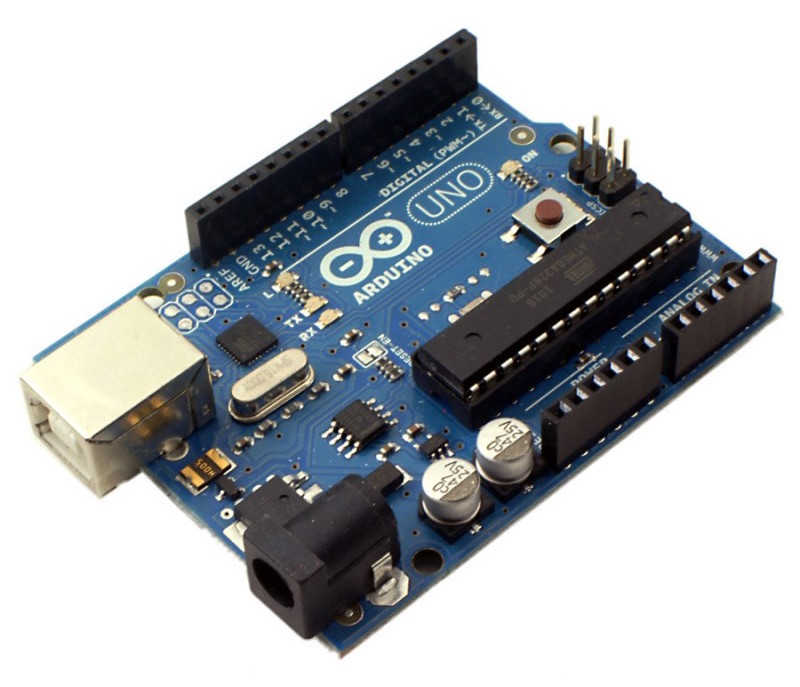
\includegraphics[width=\textwidth]{Files/arduino}
                \caption{An Arduino UNO.}
                \label{fig: arduino}
            \end{subfigure}
            ~
            \begin{subfigure}[b]{0.45\textwidth}
                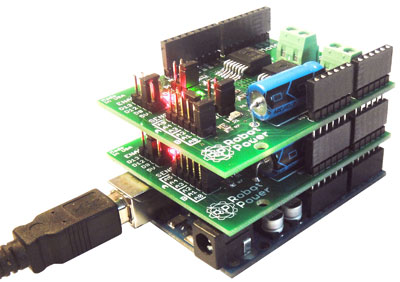
\includegraphics[width=\textwidth]{Files/arduino_with_shields}
                \caption{An Arduino with 2 \glspl{shield} attached.}
                \label{fig: arduino shields}
            \end{subfigure}
            \caption{\small (Retrieved from \citen{robotshop} on 2016--01--25)}
            \label{fig: arduino and shields}
            % \vspace{-20pt}
        \end{figure}
        The robot will need a control system to plan and control its movement, and to control the drawing tool. This system could be developed from proprietary systems or built by the group for this specific application.

        \paragraph{\gls{Arduino}} (Figure~\ref{fig: arduino}) is an open-source micro-controller system designed for embedded systems control. It can be expanded by the use of \emph{\glspl{shield}} (Figure~\ref{fig: arduino shields}), circuit boards designed to attach to header pins on the primary micro-controller board to created stacks of circuits with different functions. This would allow us to build a control system for the robot using pre-designed circuits. \Glspl{shield}, which can be bought from many electronics suppliers, are available to add bluetooth, GPS, motor control, and many other functions to the primary circuit.\\
        There is a large online community supporting the \gls{Arduino} project, which could be leveraged to solve programming difficulties if they arise. The \gls{Arduino} project provides an integrated development environment (IDE); the \gls{Arduino} is programmed using a language based on the C and C++ languages.
        \paragraph{Netduino} is a variant of the \gls{Arduino} which runs on Microsoft's .NET framework. The online support community for this system is smaller, although some group members (\AG, \LY) have a pre-existing familiarity with the .NET framework.\\

        \todo[inline]{electronics: rework the following paragraphs}
        \paragraph{Raspberry Pi}is a small single-board computer developed in the UK to promote access to computer science education in schools. Because on this, the platform is already widely used in an educational setting and thus would allow this project to be more easily integrated into the teaching of computer science. The computer itself is low-cost (<\pounds{50}\todo{check the price of Raspberry Pi}).\\
        The Raspberry Pi Foundation also produce smaller versions of the Raspberry Pi computer which are designed for use in embedded systems. These boards are less customizable than the Arduino system. However, it is compatible with the Python language, which has an extensive support community online and is familiar to all the group, as well as C, C++, Java, and others.

        \paragraph{A micro-controller} integrated circuit could be used in a purpouse-built system to control the robot. This would require the design of all the supporting electronics. The microprocessor would need to be programmed in a low-level assembly language or a language designed specifically for the micro-controller product we use.\\
        These components would be cheaper than commercially available systems, but would require much more electronics design work and fabrication.

        \mySubsection{Power}{\SSB}\label{outline: power}
            The \gls{Arduino} requires a supply voltage of \SIrange{7}{12}{\volt}. The motors will also require a power supply of \SIrange{5}{12}{\volt}. There are many different types of battery, several of which are appropriate for the robot:

            \paragraph{Single-use alkaline} batteries are common-place and cheap. They come in a variety of sizes and capacities. These batteries must be disposed of after use and can only source small currents (typically no more than 1A). \SI{9}{\volt} PP3 batteries are particularly popular for electronics projects due to their regular shape and convenient connections.
            \paragraph{Rechargeable alkaline or nickel-based} batteries can be re-used. They are often more efficient than their single-use counterparts.
            \paragraph{Lithium Polymer} batteries are often used for remote-controlled vehicles. They have a very high energy-density and can source high currents (>\SI{10}{\ampere}). This makes them particularly suited to powering small vehicles. These batteries are also rechargeable and have short charging times.

            \paragraph{}In order to allow the motors to sink high currents without affecting the supply voltage to the micro-controller, separate power supplies are used for each system: the \gls{Genuino}, the GPS shield and the \gls{magnetometer} (the control system); and the motors and \glspl{servo} (the output system). The lithium polymer batteries are the best choice for the motors since they can source the required currents and are light-weight. The capacity of the battery for the output system is a matter of cost; a high-capacity battery is more convenient but will be more expensive.\\
            The simplest power source for the control system is a \SI{9}{\volt} PP3 battery. The output system is driven by a \SI{7.4}{\volt} \SI{1500}{\milli\ampere\hour} lithium polymer battery\footnote{\pounds{12.00} from Component Shop \textsc{URL:} \url{www.componentshop.co.uk}~~~~\texttt{SKU: LN215}}. This can supply a continuous current of up to \SI{52.5}{\ampere} and can drive both motors at maximum power for 23 minutes. The control and output systems must have a common ground (\SI{0}{\volt}) connection.

\mySection{User interface}{writer TBA}
    \towrite{interface}


\section{Summary and decisions}
    \towrite{summary and decisions}
    \myBlindSubsection{Aims and motivations}{\AH}
    It was agreed by the group that the aim of this project would be the produce a sand art--drawing robot for educational purposes. The intention being that the final product may be utilised to teach pupils, of primary school age, the basic steps involved in coding.
    The children would input a design, using preliminary coding language, into an interface. The children would have to consider the steps involved in producing their desired image and input the details in a manner that a computer can understand. The group's robot would then reproduce this design in the sand. 




    \myBlindSubsection{Drawing tool}{writer TBA}


    \myBlindSubsection{Electronics platform and guidance system}{writer TBA}

    Separate power supplies are used for the control system and the motors. The power source for the control system is a \SI{9}{\volt} PP3 battery. The motors are driven by a \SI{7.4}{\volt} \SI{1500}{\milli\ampere\hour} lithium polymer battery.


    \mySubsection{Outline specification}{\textsc{Whole Group}}\label{outline specification}
        \begin{enumerate} %Reference items in this list using \refspec{drawing size} etc.
            \subsubsection{The project}
            \item We shall design and build a prototype robot to draw 2d line drawings in sand.\label{spec: draw}
            \item The robot shall take input from a user which it shall translate into instructions to draw the picture;\label{spec: take input}
            \item the drawings should be ??? \todo{how big will the drawings be?} in size; \label{spec: drawing size}
            \item the robot should be for educational uses. \label{spec: education}

            \subsubsection{Control systems}
            \item The robot shall be controlled with a \gls{Genuino} 101; \label{spec: arduino}
            \item the robot shall use \gls{GPS} for guidance; \label{spec: gps}
            \item the robot should detect objects in front of it. The robot should not collide with objects; \label{spec: detect objects}
            \item the robot should circumvent obstacles.\label{spec: circumvent}

            \subsubsection{The robot hardware}
            \item The robot shall move across the sand using ???\todo{how will it move?}; \label{spec: movement}
            \item the robot shall use ??? \todo{how will it draw?} to draw the images; \label{spec: tool}
            \item the robot shall be built from ??? \todo{what will it be built from?}; \label{spec: material}
            \item the robot shall have dimensions equal to or less than ($56 \times 45 \times 25$) cm. \label{spec: robot size}

            \subsubsection{Safety}
            \item The robot shall have an emergency shut-down switch; \label{spec: kill switch}
            \item the robot should indicate operating faults to the user; \label{spec: error indicator}
            \item the robot should have documentation and instructions for end users. \label{spec: documentation}
        \end{enumerate}
